\subsubsection{Assignment description}
The main point of focus of this project is to compare the pthreads and openCilk multi-threading systems through a real life application.
The main points of comparison are functionality, ease of use and performance, of the two multi-threading systems. The project uses C++ in
order to be compatible with the uint256\_t library but it is developed using structured programming logic. The code for this assignment 
can be found in \href{https://github.com/Billkyriaf/pds_assignment_4}{this} GitHub repository.

\subsubsection{The real life problem}
The problem used for this comparison is file compression using the Huffman algorithm. The Huffman algorithm is a lossless data compression algorithm. 
It is a variable length code algorithm, meaning that the length of the code is not fixed. The algorithm is based on the frequency of the characters in
the file. The more frequent a character is, the shorter the code for that character will be. The algorithm performs best when the distributions of the 
frequencies is not uniform. For this reason the best compression is achieved on text files with natural language. 

The natural language uses only part of the 8bit ASCII code. A typical frequency distribution of the characters in a text file is shown in the figure below.

\begin{center}
    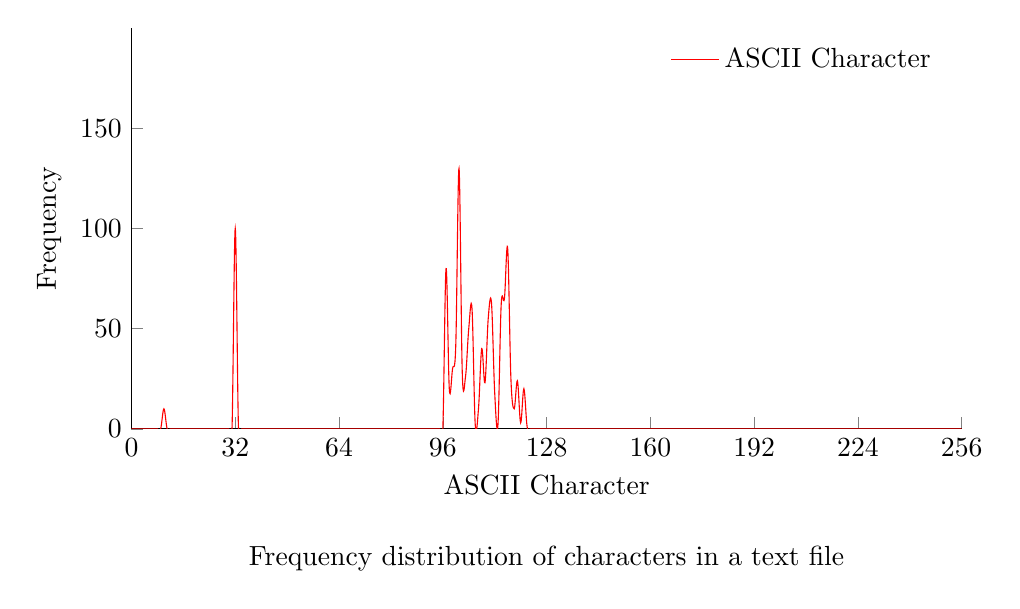
\begin{tikzpicture}
        \begin{axis}[
            title style={at={(0.5,0)},anchor=north,yshift=-45pt},
            title={Frequency distribution of characters in a text file},
            axis y line*=left,
            axis x line*=bottom,
            ylabel={Frequency},
            xlabel={ASCII Character},
            ymin=0, ymax=200,
            xmin=0, xmax=256,
            xtick={0,32,64,96,128,160,192,224,256},
            ytick={0,50,100,150},
            width = \textwidth,
            height = 0.55\textwidth,
            legend style={draw=none},
        ]
        
        \addplot[
            smooth,
            tension=0.6,
            color = red,
            ]
            coordinates {
            (0,0)(1,0)(2,0)(3,0)(4,0)(5,0)(6,0)(7,0)(8,0)(9,0)(10,10)(11,0)(12,0)(13,0)(14,0)(15,0)(16,0)(17,0)(18,0)(19,0)(20,0)(21,0)(22,0)(23,0)(24,0)(25,0)(26,0)(27,0)
            (28,0)(29,0)(30,0)(31,0)(32,100)(33,0)(34,0)(35,0)(36,0)(37,0)(38,0)(39,0)(40,0)(41,0)(42,0)(43,0)(44,0)(45,0)(46,0)(47,0)(48,0)(49,0)(50,0)(51,0)(52,0)(53,0)(54,0)
            (55,0)(56,0)(57,0)(58,0)(59,0)(60,0)(61,0)(62,0)(63,0)(64,0)(65,0)(66,0)(67,0)(68,0)(69,0)(70,0)(71,0)(72,0)(73,0)(74,0)(75,0)(76,0)(77,0)(78,0)(79,0)(80,0)(81,0)
            (82,0)(83,0)(84,0)(85,0)(86,0)(87,0)(88,0)(89,0)(90,0)(91,0)(92,0)(93,0)(94,0)(95,0)(96,0)(97,80)(98,20)(99,30)(100,42)(101,130)(102,28)(103,26)(104,50)(105,60)
            (106,2)(107,10)(108,40)(109,23)(110,55)(111,63)(112,18)(113,2)(114,62)(115,65)(116,90)(117,25)(118,10)(119,24)(120,3)(121,20)(122,1)(123,0)(124,0)(125,0)(126,0)(127,0)(128,0)(129,0)(130,0)
            (131,0)(132,0)(133,0)(134,0)(135,0)(136,0)(137,0)(138,0)(139,0)(140,0)(141,0)(142,0)(143,0)(144,0)(145,0)(146,0)(147,0)(148,0)(149,0)(150,0)(151,0)(152,0)(153,0)
            (154,0)(155,0)(156,0)(157,0)(158,0)(159,0)(160,0)(161,0)(162,0)(163,0)(164,0)(165,0)(166,0)(167,0)(168,0)(169,0)(170,0)(171,0)(172,0)(173,0)(174,0)(175,0)(176,0)
            (177,0)(178,0)(179,0)(180,0)(181,0)(182,0)(183,0)(184,0)(185,0)(186,0)(187,0)(188,0)(189,0)(190,0)(191,0)(192,0)(193,0)(194,0)(195,0)(196,0)(197,0)(198,0)(199,0)
            (200,0)(201,0)(202,0)(203,0)(204,0)(205,0)(206,0)(207,0)(208,0)(209,0)(210,0)(211,0)(212,0)(213,0)(214,0)(215,0)(216,0)(217,0)(218,0)(219,0)(220,0)(221,0)(222,0)
            (223,0)(224,0)(225,0)(226,0)(227,0)(228,0)(229,0)(230,0)(231,0)(232,0)(233,0)(234,0)(235,0)(236,0)(237,0)(238,0)(239,0)(240,0)(241,0)(242,0)(243,0)(244,0)(245,0)
            (246,0)(247,0)(248,0)(249,0)(250,0)(251,0)(252,0)(253,0)(254,0)(255,0)(256,0)
            };
            \legend{ASCII Character}
            
        \end{axis}
    \end{tikzpicture}
\end{center}

It is clear that the most frequent characters are the letters of the alphabet. Using the Huffman coding the symbols for the most frequent characters are less than the 
original 8bits of the ASCII code. Replacing the characters with those symbols will result in a smaller file size.

\subsubsection{Huffman coding significance}

The huffman algorithm is widely used in all the mainstream compression formats. It is especially effective in the compression of images, text and audio files. It provides
lossless compression, meaning that the original file can be reconstructed from the compressed file. These reasons have lead in the widespread use of the huffman algorithm.
Because Huffman algorithm is a core element of many compression algorithms, speeding it up is very desirable, as many application will benefit from it. 
